
\section{INTRODUCCIÓN}
\subsection{Introducción}
En los últimos años, gracias al gran desarrollo tecnológico que se ha vivido tanto a nivel de computo (mejorando la eficiencia y el uso de los recursos disponibles) como a nivel de transmisión de datos (mejorando las comunicaciones), ha permitido a las organizaciones el almacenamiento de una gran cantidad de información.

Esto se debe a que, como se pueden observar en las siguientes figuras (\ref{fig:procPerformance} y \ref{fig:bandwidth-growth}), las millones de instrucciones por segundo (MIPS) que realiza un procesador (relacionado con el tiempo de cómputo) y la velocidad de transmisión de datos en bits por segundo (BPS) han crecido a lo largo de los últimos años \cite{Nielsen2018}.

\begin{figure*}[htb]
	\centering
	\caption{Velocidad Procesador (MIPS) a lo largo del tiempo. (Fuente: Kurzweil http://www.kurzweilai.net)}
	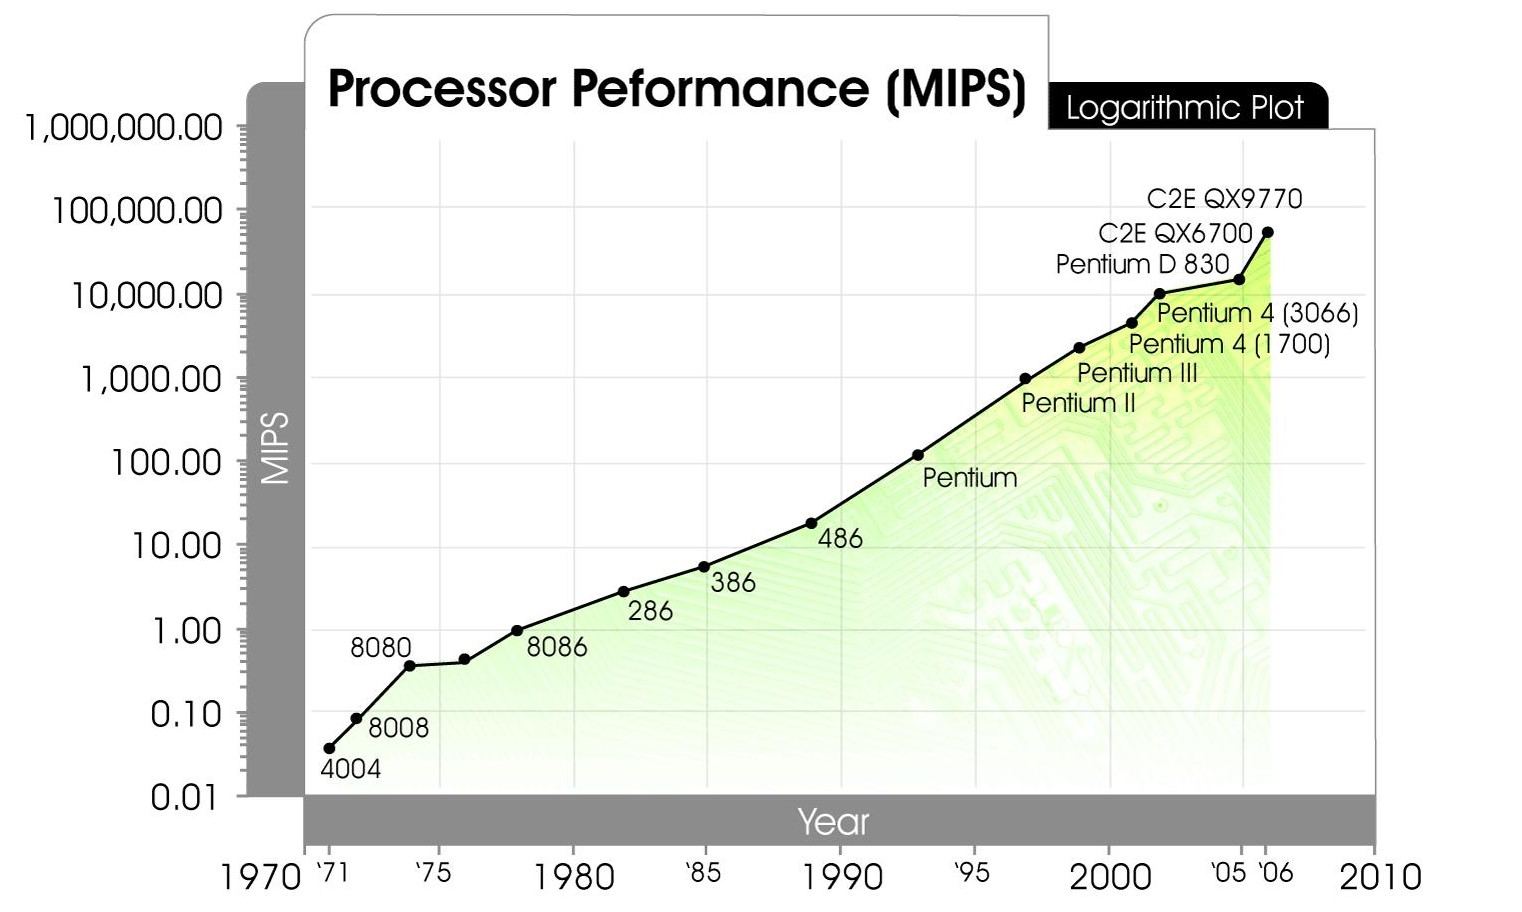
\includegraphics[width=0.6\textwidth]{recursos/processor_performance}
	\label{fig:procPerformance}
\end{figure*}
\FloatBarrier
\begin{figure*}[htb]
	\centering
\caption{Velocidad de transferencia a lo largo del tiempo. (Fuente: Nielsen Norman Group)}
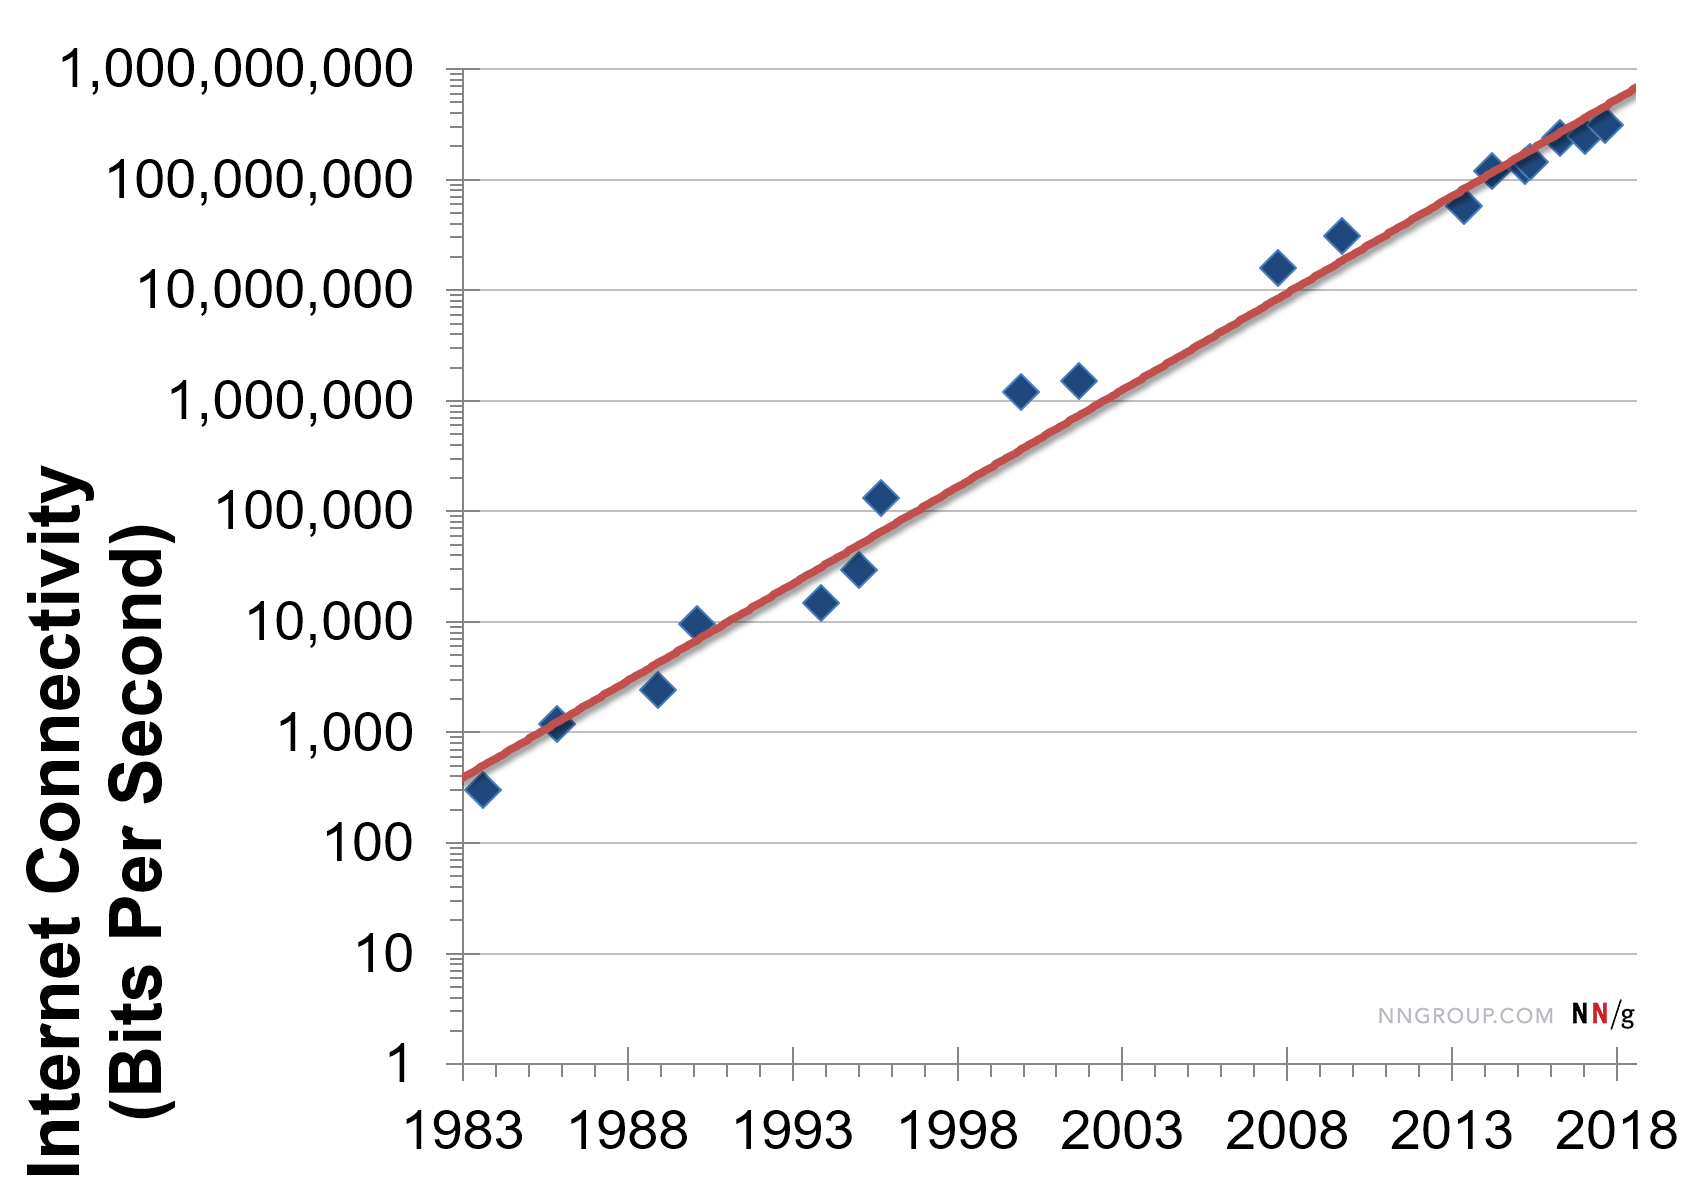
\includegraphics[width=0.5\textwidth]{recursos/bandwidth-growth-nielsen-law}
\label{fig:bandwidth-growth}
\end{figure*}
\FloatBarrier
Para comprender mejor este gran volumen de información, es necesario utilizar métodos, técnicas, herramientas además de personas con conocimientos (formando todas esta un vínculo estrecho) que permita y ayude a explotar, investigar, predecir y obtener información relevante para tomar decisiones de forma adecuada.

Para descubrir la información en estos grandes volúmenes de datos, es necesario abordar el concepto de minería de datos.  Según \citeA{martinez2016mineria}, la minería de datos es el ``proceso que permite transformar información en conocimiento útil para el
negocio, a través del descubrimiento y cuantificación de relaciones en una
gran base de datos". La minería de datos aplica técnicas estadísticas y matemáticas para poder obtener esta información implícita en los datos.



Algunas de las aplicaciones de la minería de datos según \cite{riquelme2006mineria} son:  comercio y banca, medicina y farmacia, seguridad y detección de fraude, astronomía, geología, minería, agricultura, pesca, ciencias ambientales y ciencias sociales.


\subsection{Contexto}
La organización educativa no ha quedado ajena a estas necesidades de una mejor comprensión de los datos. Según \citeA{romero2010educational} la minería de datos educativa (EDM) se encarga del desarrollo de métodos para explotar los datos del entorno educativo y entender mejor a los estudiantes y las herramientas que se utilizan para el aprendizaje de estos.

Por un lado, tanto el software educativo como las bases de datos institucionales, han generado una gran cantidad de datos acerca de alumnos, reflejando el aprendizaje de estos a lo largo del tiempo. \cite{romero2010educational}

Por otro lado, el uso de pedagógico de Internet (eLearning), ha generado también grandes cantidades de datos acerca de la enseñanza-aprendizaje (técnicas, herramientas, etc). \cite{romero2010educational}.

"Toda esta información es una mina de oro, en el contexto educativo". \cite{romero2010educational}.

El proceso de EDM convierte los datos en bruto,obtenidos de sistemas educativos en información útil que puede tener un gran impacto en las investigaciones y practicas educativas. \cite{romero2010educational}

No obstante, como se indica en el libro de \cite{inbook} la EDM se ha desarrollado mas lentamente que en el resto de ámbitos.

Como se puede observar en el articulo de \citeA{sin2015application} y en la figura \ref{fig:artPublicados}, el numero de artículos publicados en la conferencia internacional sobre la minería de datos ha crecido desde 2011. 

Este aumento de artículos publicados implica un aumento en el uso de la minería de datos en la educación.

\begin{figure*}[htb]
	\centering
	\caption{Artículos aceptados y publicados desde 2011. Recuperado de \protect\citeA{sin2015application}}
	\includegraphics[width=0.6\textwidth]{recursos/artPublicados}
	\label{fig:artPublicados}
\end{figure*}
\FloatBarrier

A su vez, \citeA{sin2015application}, ha categorizado los artículos publicados según su contenido en categorías que definen las distintas aplicaciones de la minería de datos en la educación. Algunas de estas categorías son: detección de comportamiento, estimación de habilidades, predicción de mejora académica, etc


\begin{comment}
Desde la Consejería de Educación de Madrid se están realizando proyectos para conseguir sacar la máxima información del gran número de datos que se poseen.


Obviamente, debido a este gran tamaño de datos, es necesario utilizar métodos, herramientas y personas con conocimientos para obtener información concreta en un tiempo legible. Desde la Consejería de Educación se quiere tener conocimientos actuales sobre la situación educativa. Un ejemplo podría ser el número de alumnos matriculados con necesidades educativas para un determinado centro de la Dirección de Área Territorial Sur. No solo eso, también podrían obtenerse alumnos de un determinado nivel educativo o incluso grupos.


%http://www.superiorinfotech.com/bidw.html
\begin{figure*}[htb]
	\centering
	\caption{
		Arquitectura de un almacén de datos. Recuperado de: Superior Information Technology.
	}
	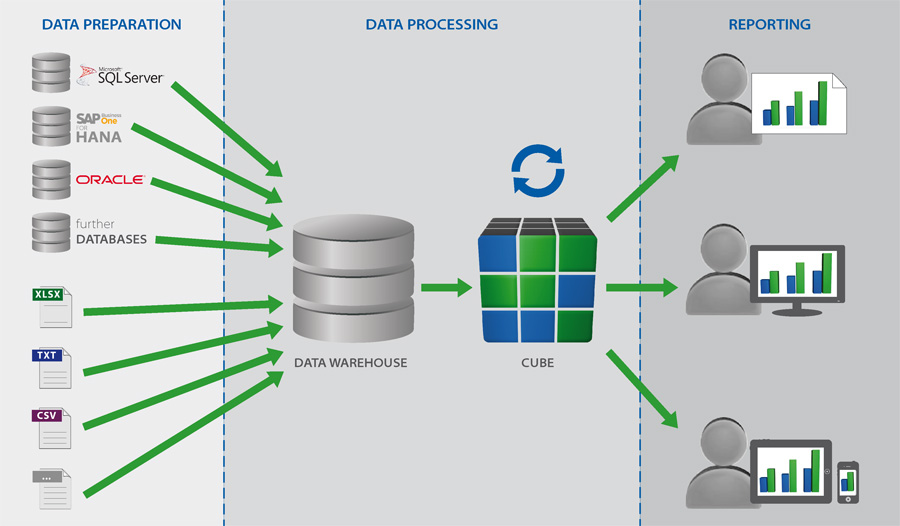
\includegraphics[width=0.6\textwidth]{recursos/arquitecturaDatawarehouse}
	\label{fig:ArqDWH}
\end{figure*}

En la figura \ref{fig:ArqDWH} se pude observar la arquitectura de un almacén de datos. Mediante esta arquitectura, los usuarios finales pueden obtener mucha información sin necesidad de realizar consultas complejas a bases de datos.

No obstante, mostrar la información actual o pasada no es suficiente. La Consejería de Educación también requiere obtener datos futuros. En este aspecto, la Consejería necesita saber cuántos alumnos podrán matricularse en el futuro, con el objetivo de destinar recursos a los centros.
Por tanto, será necesario utilizar técnicas predictivas. Estas técnicas se pueden usar perfectamente en la Consejería puesto que requieren una gran cantidad de datos para realizar pronósticos ajustados, en este sentido, la Consejería tiene un gran histórico de años anteriores.
\end{comment}

\subsection{Objetivos}
Con este TFM se propone dar una solución a un problema actual de una unidad (de Secundaria) de la Consejería de Madrid, mediante el uso de herramientas y métodos flexibles que automaticen dichas tareas y proponga, además, nuevas variables o factores que puedan influir en la toma de decisión. 

Los objetivos que se quiere cumplir con este TFM son los siguientes:
\begin{itemize}
	\item Seleccionar variables que interesen estudiar y que aporten valor en el desarrollo de este TFM.
	\item Obtener modelos que se ajusten correctamente a los datos.
	\item Probar distintos modelos y seleccionar aquellos que aporten mayor precisión en la predicción. 
	\item Realizar predicciones con datos existentes.
\end{itemize}

\subsection{Metodología}
El proceso o metodologia llevado a cabo en este TFM ha seguido las siguientes fases:
\begin{enumerate}
	\item En primer lugar, se ha detectado una determinada necesidad en una unidad de la Consejería de Educación.
	\item Una vez detectada la necesidad, se han realizado reuniones con dicha unidad para obtener la mayor información posible acerca de sus necesidades y la forma en la que satisfacerlas. Antes de comenzar la investigación, se debe tener un claro conocimiento sobre las necesidades existentes y establecer un plan de acción.
	\item Una vez se tiene claro cual es la necesidad, se va a realizar una propuesta para poder satisfacer las necesidades de la unidad.
	\item La propuesta establecida debe ser validada por la propia unidad.
	\item Una vez validada la propuesta, se deben estudiar distintos modelos. Se debe analizar cual de los modelos es el que mayor precisión obtiene.
	\item Por ultimo, se debe validar el modelo seleccionado y realizar las predicciones correspondientes con los datos de la unidad.
%	\item Del estado del arte, se van a tener nuevas metodologías, técnicas y  herramientas que ayuden a resolver el problema del estudio. Por tanto, se deberá recopilar dicha información para llevar a cabo la investigación.
%	\item Dicha información recopilada se debe acotar respecto a las necesidades del problema que se necesita resolver en la investigación, y se debe llevar a cabo en esta.
%	\item Aplicando dichos conocimientos (metodologías, técnicas y herramientas), se obtienen unos resultados, que se van a interpretar, dando lugar a nuevos conocimientos del caso estudiado.
\end{enumerate}

%Esta norma nos va a guiar en la realización de la investigación siguiendo una serie de etapas que parte de la identificación de las necesidades hasta llegar a los resultados deseados.

%Para ello se partirá de una serie de reuniones con los responsables de la unidad, para entender las necesidades y problemas. Una vez que se tienen las necesidades, se deben analizar y localizar que fuentes de datos se van a utilizar. Además, se estudiará las herramientas que la unidad utiliza para realizar estas predicciones y además se estudiaran las variables que utilizan.

%A partir de la fuente de datos, se deberá realizar un análisis exploratorio (o descriptivo) de estos. Este análisis nos indicara que variables son más importantes y cuales incluso se podrían desechar.  Este análisis se va a tener en cuenta a la hora de realizar el modelado de datos.

%Una vez que se ha realizado el modelado de datos, aplicando diversos algoritmos, se elegirá aquel que mejores resultados aporte (mayor precisión en la predicción). Posteriormente, teniendo en cuenta cual es el mejor modelo, se podrán realizar predicciones de los propios datos.

%Después se seleccionarán aquellos datos que se consideran importantes para realizar las labores de predicción. Para realizar la selección, se debe estudiar los mecanismos ya existentes en esta Unidad de Secundaria para obtener aquellos en uso. Una vez que se han seleccionado los datos, se va a realizar un tratamiento de estos para poder utilizarlos en las nuevas herramientas.

%Por último, se van a aplicar modelos predictivos y se van a seleccionar aquellos que mayor precisión aporten con dichos datos.

\subsection{Organización del TFM}
La estructura que se va a seguir en el TFM va a ser la siguiente:
\begin{itemize}
	\item \textbf{Capitulo 1. Introducción:} En el primer capítulo se van a definir las necesidades existentes que justifican el desarrollo de este trabajo. También se va a definir los objetivos que se persiguen con la realización de este. Por último, se presenta la estructura que tendrá el presente documento.
	\item \textbf{Capitulo 2. Justificación teórica:} En este segundo capítulo se va a realizar una investigación sobre el estado de la cuestión. Se va a realizar un estudio sobre los métodos, modelos y usos de la minería de datos en el ámbito educativo. 
	\item \textbf{Capitulo 3. Propuesta de intervención:} En este tercer capítulo se va a plantear una solución al problema existente. 
	\item \textbf{Capitulo 4. Diseño de la investigación:} Este capítulo va a definir los pasos que se seguirán en la realización de un proyecto de minería de datos. Se van a detallar también las tareas que se van a desempeñar en cada uno de los pasos.
	\item \textbf{Capitulo 5. Conclusiones:} En este capítulo se van a detallar las conclusiones obtenidas a partir de los resultados alcanzados.
\end{itemize}




